%%%%%%%%%%%%%%%%%%%%%%%%%%  phdsymp_sample2e.tex %%%%%%%%%%%%%%%%%%%%%%%%%%%%%%
%% changes for phdsymp.cls marked with !PN
%% except all occ. of phdsymp.sty changed phdsymp.cls
%%%%%%%%%%                                                       %%%%%%%%%%%%%
%%%%%%%%%%    More information: see the header of phdsymp.cls   %%%%%%%%%%%%%
%%%%%%%%%%                                                       %%%%%%%%%%%%%
%%%%%%%%%%%%%%%%%%%%%%%%%%%%%%%%%%%%%%%%%%%%%%%%%%%%%%%%%%%%%%%%%%%%%%%%%%%%%%%


%\documentclass[10pt]{phdsymp} %!PN
\documentclass[twocolumn]{phdsymp} %!PN
%\documentclass[12pt,draft]{phdsymp} %!PN
%\documentstyle[twocolumn]{phdsymp}
%\documentstyle[12pt,twoside,draft]{phdsymp}
%\documentstyle[9pt,twocolumn,technote,twoside]{phdsymp}

\usepackage[english]{babel}       % Voor nederlandstalige hyphenatie (woordsplitsing)

\usepackage{graphicx}                   % Om figuren te kunnen verwerken
\usepackage{graphics}			% Om figuren te verwerken.
\graphicspath{{figuren/}}               % De plaats waar latex zijn figuren gaat halen.

\usepackage{times}

\hyphenation{si-mu-la-ted re-a-lis-tic packets really in-clu-ding}

\def\BibTeX{{\rm B\kern-.05em{\sc i\kern-.025em b}\kern-.08em
    T\kern-.1667em\lower.7ex\hbox{E}\kern-.125emX}}

\newtheorem{theorem}{Theorem}

\begin{document}

\title{Broadband access network for trains based on Radio-over-Fiber} %!PN

\author{Peter Dedecker}

\supervisor{Ingrid Moerman, Didier Colle, Bart Lannoo, Bart Jooris, Tom Van Leeuwen}

\maketitle

\begin{abstract}
This article tries to extend the limits of the trade off between bandwidth and velocity by proposing a new model for trains based on Radio-over-Fiber and the \textit{moving cell} concept.  This model has been tested by simulations with currently available technology.
\end{abstract}

\begin{keywords}
Radio-over-Fiber, moving cell, access network, fast moving users, wireless technologies
\end{keywords}

\section{Introduction}
\PARstart{T}{he} well known problem with broadband access networks is their trade off between bandwidth and velocity.  While a WiFi-network can support up to 54~Mbps, you have to stay in the close neighborhood of the access point.  Network technologies that allow you to move, like GSM, only support 9600 bps, or 170~kbps when using GPRS.  Their problem is that small cells are needed to provide a high bandwidth, but with small cells you have to change to another cell very frequently, which is called the handover problem.

This problem typically arises on trains: one wants to have access to a broadband internet connection at a travelling speed up to 300~km/h for high speed trains.  Today, this is possible when using a satellite connection, but there are lots of drawbacks: a long round trip time, need for a line of sight connection and a high price for a connection of e.g. only 2-4~Mbps.

In this abstract, we will first propose a model based on antennas near the railway and solve the handover problem.  This model will be tested by simulations as proof of concept and compared to traditional communication systems.


\section{Moving cell by Radio-over-Fiber: concept}

\subsection{Radio-over-Fiber}
This model was proposed earlier in \cite{paper}.  We divide the track of the train in cells.  In each cell, base stations are placed near the railway and connected with a central node by an optical fiber.  Each base station has a direct line to the central node by its own optical wavelength.  In such an optical ring the central node needs to know where the train actually is so it can send packets to the right base station by modulating it on the right wavelength.

To reduce the cost of those base stations, they need to be really simple.  This can be achieved by using \textit{Radio-over-Fiber}: the base stations are just dumb antennas, capture a whole frequency band and place it integrally and immediatly on the optical wavelength.  The actual decoding takes place in the central node.  Such antennas are called \textit{Remote Antenna Units} (RAU's) in RoF-terminology.  Those wireless signals can be decoded by the central node when the attenuation is low enough.  This is normally a fact if the length of the ring is held under 10~km.

\subsection{Moving Cell}
Normal handovers follow a fixed scenario by searching for an antenna at different frequencies.  In most wireless network standards a handover needs also to be completed by exchanging management frames.  After this, packets located in buffers at the previous antennas need to be rerouted which can take some time and obstructs fast handovers.  We can eliminate this if we define fixed frequencies for all receivers.

This can be done by generating all wireless packets in the central node.  Those packets are then placed on the right optical wavelenght so they are sent out by the right RAU on the right frequency.  When the train comes in the neighborhoud of another RAU the central has to send those downlink packets to that new RAU.

This way, the train can keep its frequency the whole track in the same optical ring and no handovers are needed anymore.  This principle, by holding the same frequency and keeping the train connected to the same logical access point in the central node, is called \textit{moving cell}.

For simplicity reasons, all trains in the optical ring have their own dedicated frequency.


\subsection{Traffic Routing}
To get downstream packets at the right RAU, the central node has to keep track of the train location.  This can easily be done by monitoring upstream packets.  The RAU that picks up the upstream packets coming from the train are likely the ones closest to the train.  When the train moves and the signals are picked up by a new RAU, this RAU will soon be the only RAU that communicates with the train.  The central node can then switch to the new RAU almost as soon as when the first packet reaches the central node by this new RAU.  Of course the central node needs to remember the previous RAU in orde to avoid switching back again in the overlap zone.

While all trains have their own dedicated channel, it is possible to support multiple trains or crossing trains at the same RAU's.  It is even possible to place more than one sender/receiver on the train, each with their own channel, to increase bandwidth.


\section{Simulation model}
The operation of this model has to be demonstrated by simulations, however this is not evident with new technology.  So we have to map it to currently available technology.

First of all, as wireless standard we choose IEEE~802.11, commonly known as WiFi, which is a cheap and easily available technology nowadays.  To approach the concept of capturing a whole frequency band, we install a number of wireless network cards in the nodes that act as RAU so we can capture a small selection of that frequency band.  There is one WiFi card needed in each RAU for each train/channel we want to support.

As an optical network is not available, we have to fall back on traditional ethernet.  By connecting the central node and the RAU's with a hub or switch and give all nodes a dedicated MAC-address, we can simulate the optical fiber where the central node can send packets to each RAU separately.  To model the RoF, the RAU's encapsulate the whole captured packet including extra information like signal/noise ratio and received power into a new ethernet packet and send it to the central.  The RAU's do not do anything with these packets except forwarding them, so they really act like dumb antennas.


\section{The actual simulations and results}
For the simulations themselves, we have chosen ns-click \cite{ns-click}.  This way, we can run click-scripts \cite{click} on nodes created and simulated by the ns {N}etwork {S}imulator \cite{ns}.

\subsection{Reference}
Of course, we want to compare our system to the classical ones, so we need a reference model.  We can compare our system to a hardware test as well as to a simulation test with the same ns-simulator.  Results for the ns-one are shown in figure \ref{2AP}.  Notice the gap where no communication is possible.

\begin{figure}[ht]
\begin{center}
	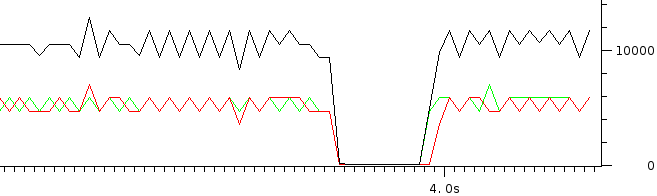
\includegraphics[width=.40\textwidth]{referentie-detail}
	\caption{\label{2AP}Detailed capture of the stream at the moment of a handover between two simulated AP's with a strong signal.  Notice the gap of 100~ms.}
\end{center}
\end{figure}


\subsection{1 train, 2 remote antenna units}
A first test scenario is created by placing two RAU's at a distance of 200~m from each other.  Each of them has a coverage range of 105~m so there is an overlap zone of 10~m.  A train passes 10~m behind the two RAU's at a speed of 40~m/s (\~144~km/h).  A UDP test stream is sent in both directions.

Results are clear: the throughput of the UDP test stream is shown in figure \ref{resultaten-1t2bs} while the network traffic between the central node and the RAU's is shown in figure \ref{RoF-1t2rau-centrale.png}.  It is clear the network connection is not broken anymore when changing to a new antenna.  In figure \ref{RoF-1t2rau-centrale.png} we can also clearly see the overlap zone of the two RAU's as the section where the blue and purple lines are not zero in together.  We have to clarify that the red and green lines are straight vertical lines, but they are shown smooth because of the stretched out figure.  You can also clearly see the traffic from the central node to the first RAU stops as soon as the first packet from the new RAU is received.


\begin{figure}[ht]
\begin{center}
	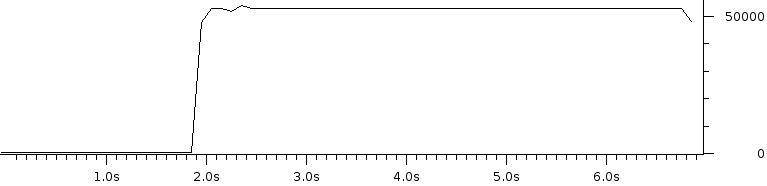
\includegraphics[width=.40\textwidth]{resultaten-1t2bs}
	\caption{\label{resultaten-1t2bs}Throughput of the UDP test stream in the RoF-model.  The network connection is not broken anymore as there is no gap.}
\end{center}
\end{figure}


\begin{figure}[ht]
\begin{center}
	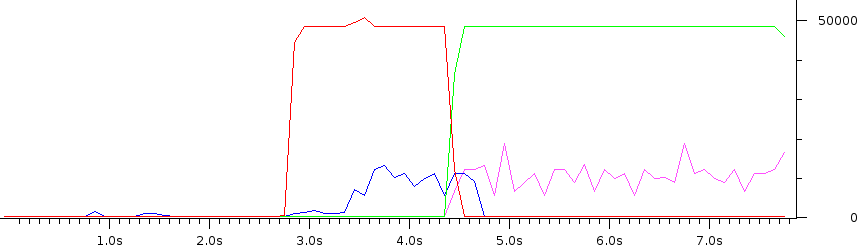
\includegraphics[width=.40\textwidth]{RoF-1t2rau-centrale.png}
	\caption{\label{RoF-1t2rau-centrale.png}Network streams in the RoF-model.  Red and green lines show the traffic from the central node to RAU1 and RAU2, blue and purple show the traffic from RAU1 and RAU2 to the central node.}
\end{center}
\end{figure}


\subsection{2 trains, 3 remote antenna units}
A second test is created by placing three RAU's at a distance of 200~m from each other and use two trains.  The first one starts at RAU1 and drives towards RAU3 while the second one makes the opposite movement.  A UDP throughput test delivers a graphs like figure \ref{resultaten-1t2bs}.  A more interesting result however is shown in figure \ref{2trein3rau}.  One can clearly see the two black peaks where both trains are in an overlap zone and their traffic is captured by two RAU's and sent to the central node together.  The other graphs look the same as in the previous one but are slightly different when both trains are in the area of RAU2 where the traffic is twice as high.

\begin{figure}[ht]
\begin{center}
	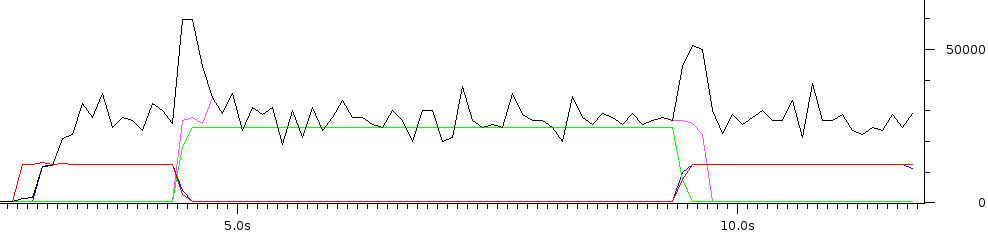
\includegraphics[width=.40\textwidth]{2trein3rau}
	\caption{\label{2trein3rau}Network streams in the RoF-model with two trains and three RAU's.  Red, green and blue lines show the traffic from the central node to RAU1, RAU2 and RAU3.  The purple one shows the traffic from RAU2 to the central node while the black line shows the total stream to the central node.}
\end{center}
\end{figure}


\section{Conclusion}
The simulation results show a nice advantage for the moving cell concept.  The traditional handover problem can be avoided so a workable model for broadband access on trains seems realistic.  But there needs to be done a lot of research to make RAU's and RoF as reliable and cheap as possible.

\nocite{*}
\bibliographystyle{phdsymp}
%%%%%\bibliography{bib-file}  % commented if *.bbl file included, as
%%%%%see below


%%%%%%%%%%%%%%%%% BIBLIOGRAPHY IN THE LaTeX file !!!!! %%%%%%%%%%%%%%%%%%%%%%%%
%% This is nothing else than the phdsymp_sample2e.bbl file that you would%%
%% obtain with BibTeX: you do not need to send around the *.bbl file        
%%
%%---------------------------------------------------------------------------%%
%
\begin{thebibliography}{1}
\bibitem{paper}
Bart Lannoo, Didier Colle, Mario Pickavet, Piet Demeester,
\newblock {\em Optical Switching Architecture to Implement Moveable Cells in a Multimedia Train Environment},
\newblock Proc. of ECOC 2004, 30th European Conf. on Optical Communication, vol. 3, pp. 344-345, Stockholm, Sweden, 5-9 Sep. 2004.

\bibitem{ns-click}
Michael Neufeld, Ashish Jain, Dirk Grunwald,
\newblock {\em Nsclick:: bridging network simulation and deployment},
\newblock http://systems.cs.colorado.edu/Networking/nsclick/

\bibitem{click}
\newblock {\em The Click Modular Router Project},
\newblock http://www.read.cs.ucla.edu/click/

\bibitem{ns}
\newblock {\em {NS} -- {N}etwork {S}imulator},
\newblock http://nsnam.isi.edu/nsnam/

\end{thebibliography}
%
%%---------------------------------------------------------------------------%%

\end{document}

%%%%%%%%%%%%%%%%%%%%%  End of phdsymp_sample2e.tex  %%%%%%%%%%%%%%%%%%%%%%%%%%%
